\section{Geometria Diferencial}

\subsection{Vetores no $\mathbb R^n$}

\subsection{Problemas}
\begin{enumerate}
    \item
        As coordenadas esféricas $r,\theta,\phi$ para o $\mathbb R^3$ são
        definidas de acordo com as seguintes equações a partir das coordenadas
        cartesianas $x,y,z$:
        \begin{align*}
            x&=r\sin\theta\cos\phi\\
            y&=r\sin\theta\sin\phi\\
            z&=r\cos\theta
        \end{align*}
        e podem ser visualizadas como na figura abaixo.
        \begin{figure}[H]
            \centering
            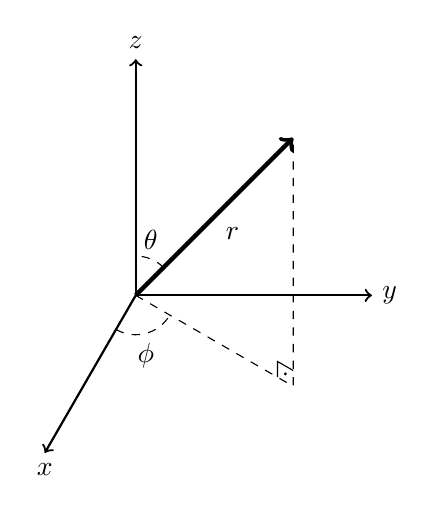
\begin{tikzpicture}
                \draw[thick,->]
                    (0,0) -- ({-2*tan(30)},-2) node[below]{$x$};
                \draw[thick,->]
                    (0,0) -- (3,0) node[right]{$y$};
                \draw[thick,->]
                    (0,0) -- (0,3) node[above]{$z$};
                \draw[ultra thick, ->]
                    (0,0) -- node[pos=0.5, below right] {$r$} (2,2);
                \draw[dashed]
                    (0,0) -- (2,{-2/tan(60)}) -- (2,2);
                \draw
                    (1.8,{-1.8/tan(60)}) -- (1.8,{-1.8/tan(60)+0.2})
                    -- (2,{-2/tan(60)+0.2});
                \fill
                    (1.9,{-1.9/tan(60)+0.1}) circle (0.02);
                \draw[dashed]
                    ({0.5*cos(240)},{0.5*sin(240)})
                    arc (240:330:0.5) node[pos=0.5,below] {$\phi$};
                \draw[dashed]
                    ({0.5*cos(45)},{0.5*sin(45)})
                    arc (45:90:0.5) node[pos=0.5,above] {$\theta$};
            \end{tikzpicture}
        \end{figure}

        Note que estas parametrizam o espaço usando $[0,\infty)\times[0,\pi]
        \times[0,2\pi)$. Encontre, como função de $r,\theta,\phi$
        \begin{enumerate}
            \item
                A base $e_r,e_\theta,e_\phi$ em termos da base $e_x,e_y,e_z$
                \answer{
                    $e_r=\sin\theta(\cos\phi e_x+\sin\phi e_y)+\cos\theta e_z$
                    \par$e_\theta=
                    r(\cos\theta(\cos\phi e_x+\sin\phi e_y)-\sin\theta e_z)$
                    \par$e_\phi=r\sin\theta(-\sin\phi e_x+\cos\phi e_y)$}
            \item
                A métrica para as coordenadas esféricas, supondo a métrica
                euclideana para as cartesianas.
                \answer{
                    $g=\left(\begin{matrix}
                        1&0&0\\
                        0&r^2&0\\
                        0&0&r^2\sin^2\theta
                    \end{matrix}\right)$
                }
            \item
                Vemos a partir do item anterior que as coordenadas esféricas
                formam um sistema ortogonal. Encontre os versores $\hat r,\hat
                \theta,\hat\phi$ em termos dos versores $\hat x, \hat y,\hat z$.
                \answer{
                    $\hat r=
                    \sin\theta(\cos\phi\hat x+\sin\phi\hat y)+\cos\theta\hat z$
                    \par$\hat\theta=
                    \cos\theta(\cos\phi\hat x+\sin\phi\hat y)-\sin\theta\hat z$
                    \par$\hat\phi=-\sin\phi\hat x+\cos\phi\hat y$
                }
        \end{enumerate}
\end{enumerate}
